\section{Overview}

% \section{To Solve is To Search}

The main source of seraching is similarity and familiarity.

Give me a point on $f(x) = \dfrac{3}{2} x + 1$, the initial responce would be the point $(2, 4)$, the reason is not defined in the strict instruction, but in the process of human likeness of similarity.

\subsection{Core Concepts in Solving a Problem}

This is more convinient to say about solving a typical problem. To say it as typica l, I am neither refer it as a knee-jerk reaction, nor as a tough math problem requiring hours to solve, but maybe take a few minutes no longer than half an hour to solve.

Here are some important notes:

\begin{enumerate}
  \item \textbf{Parse} the problem string into an array of \textbf{signals}.
  \item \textbf{Signals} contains the conditions and the purposes of the problem.
  \item \textbf{Signals} are processed by \textbf{rules of transformations}.
  \item \textbf{Transformations} has many kinds, notably, \textbf{Mechanical Transformation}, \textbf{On-Purpose Transformation} and \textbf{Heuristics Transformation}.
  \item \textbf{Mechanical} one is the process of seeing A, transform something to B.
  \item \textbf{On-Purpose Transformation} is the procee of to see A, transform something to B.
  \item \textbf{Heuristics Transformation} is in the middle of the above twos. It always involves nondeterministic path choosing. The principle of heuristics is that by trying one particular avenue, it will save much computation comparing to other options.
  \item The sequences of the transformation will lead you from conditions as the starting point to purposes.
\end{enumerate}

\begin{figure}
  \centerline{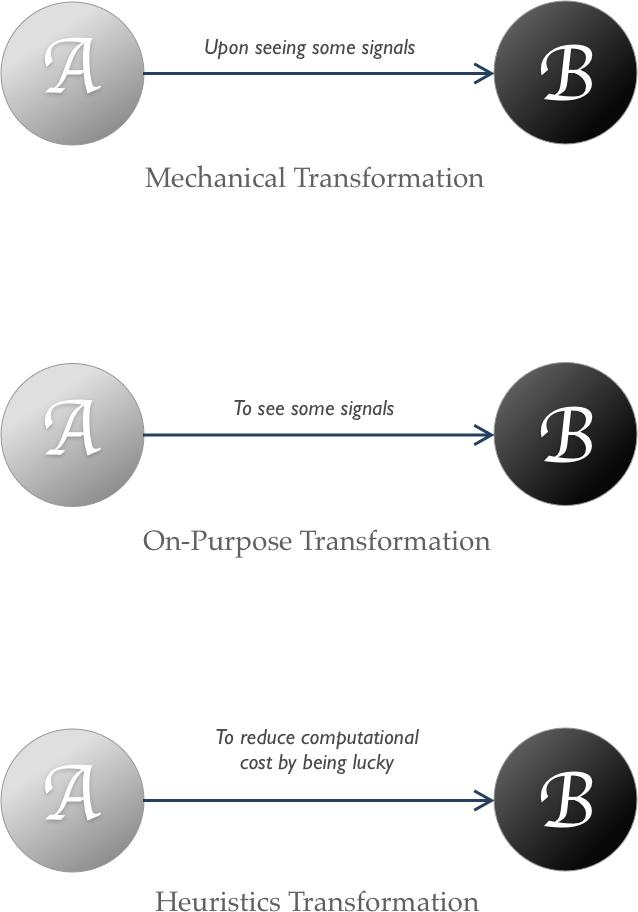
\includegraphics[width=0.8\linewidth]{img/transformations.png}}
  \caption{Types of Transformation}
  \label{fig:transformation}
\end{figure}

%
% \begin{figure}
%   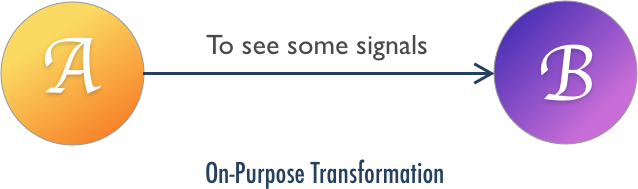
\includegraphics[width=\linewidth]{img/purpose.png}
%   \caption{Computation Models}
%   \label{fig:purpose}
% \end{figure}
%
% \begin{figure}
%   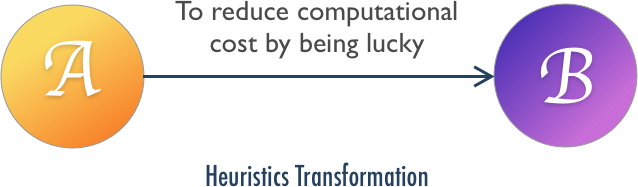
\includegraphics[width=\linewidth]{img/heuristics.png}
%   \caption{Computation Models}
%   \label{fig:heuristics}
% \end{figure}


\subsection{Examples to Find a Path}

\begin{example}
  Simplify: $ 4\cos 50^\circ - \tan 40^\circ $
\end{example}
